\documentclass[12px]{article}
\setlength{\parindent}{4em}
\usepackage[margin=2cm]{geometry}
\usepackage{graphicx}
\usepackage{amsmath}
\usepackage{amssymb}
\usepackage{enumerate}
\usepackage{multicol}
\usepackage{pifont}
\linespread{1.5}
%Title%
\begin{document}
\begin{center}
    \Large\textbf{Section 2.5 Continuity, I.V.T. and Limits at Infinity}
\end{center}

\begin{enumerate}
    %Continuity%
    \item Continuity
    \begin{enumerate}[(1)]
        %Recall%
        \item Recall:\ Limits\\
        \hspace*{2em}We have learned how to find the limits of the function at specific point, while doing so, you might find that some of the limits are not equal to the definition of the function at the same points. So we are going to introduce the concept of "Continuity".\\
        %Definition%
        \item Definition\\
        \hspace*{2em}Continuity means the function is defined at $(a, f(a))\ (a\in Domain\ of\ f(x))$, and the limits approach $a$ exist and is equal to $f(a)$. We can enumerate 3 requirements of the definition:
        \begin{multicols}{3}
            \begin{enumerate}
                \item $f(a)$ is defined
                \item $\lim\limits_{x\to a}f(x)$ exists
                \item $\lim\limits_{x\to a}\, =f(a)$
            \end{enumerate}
        \end{multicols}
        \begin{multicols}{2}
            \begin{center}
                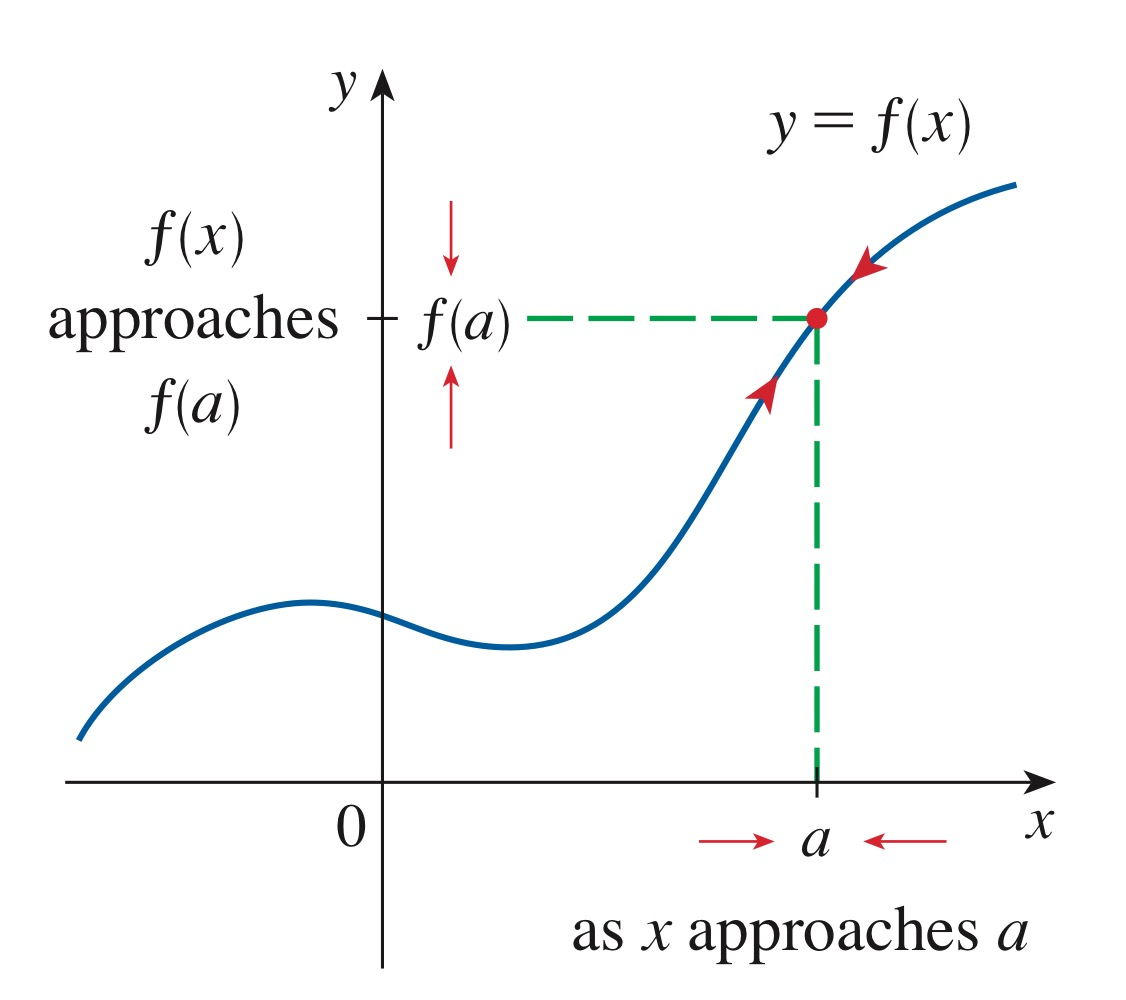
\includegraphics[width=6cm]{Continuity.JPG}\\
            \end{center}
            \begin{center}
                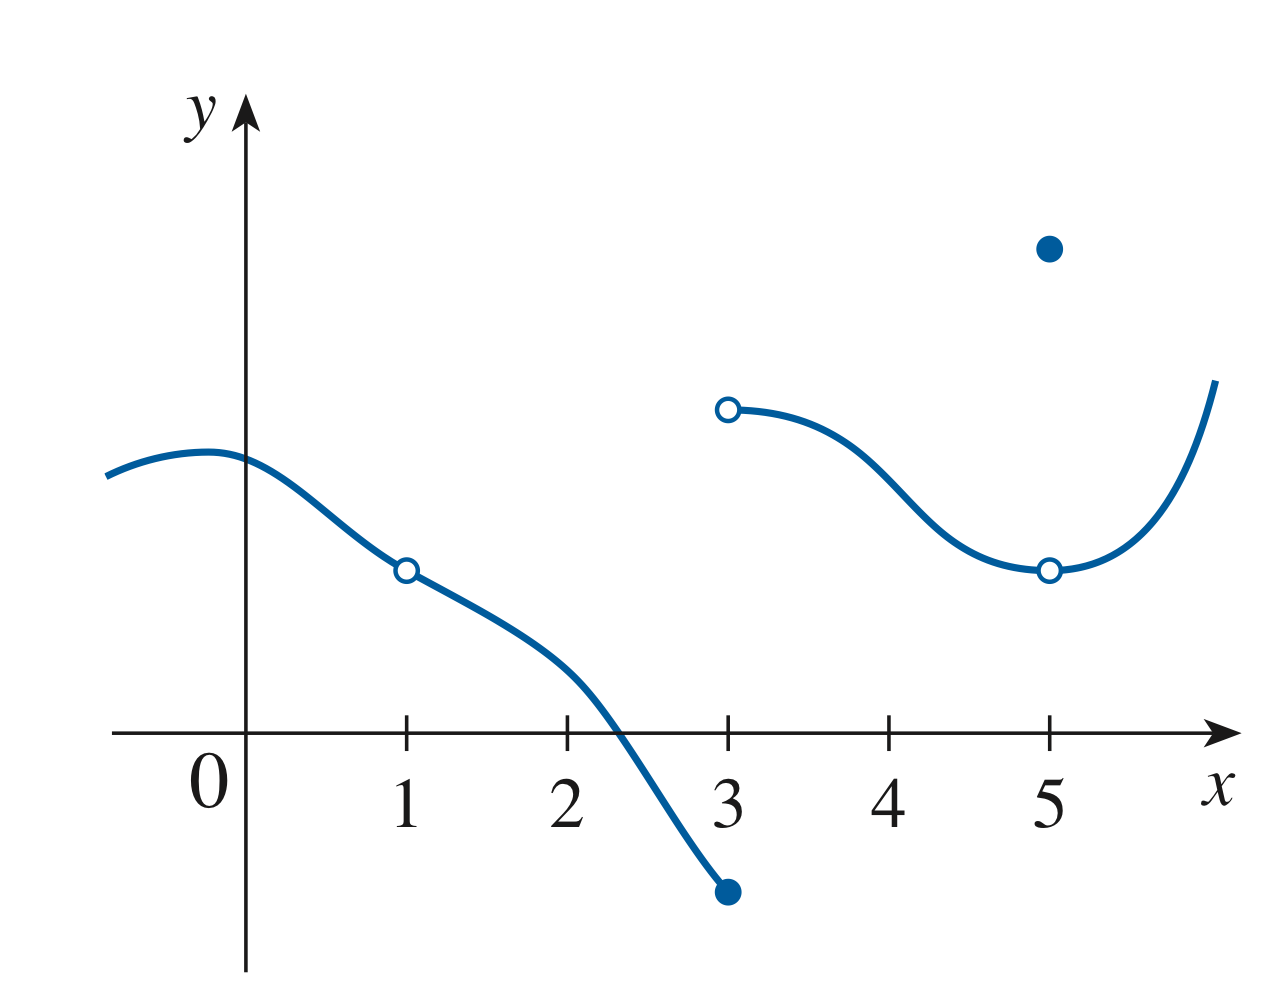
\includegraphics[width=6cm]{Discontinuity.png}\\
            \end{center}
        \end{multicols}
        %Discontinuity%
        \item Type of Discontinuity
        \begin{multicols}{4}
            \begin{enumerate}
                \item Hole
                \item Infinity
                \item Break
                \item Oscillation
            \end{enumerate}
        \end{multicols}
        \begin{multicols}{4}
            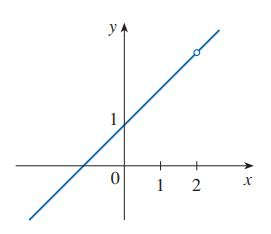
\includegraphics[width=3.5cm]{Hole.png}\\
            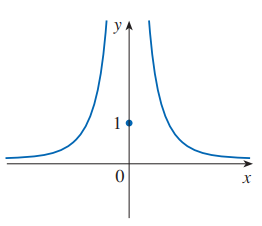
\includegraphics[width=3.5cm]{Infinite.png}\\
            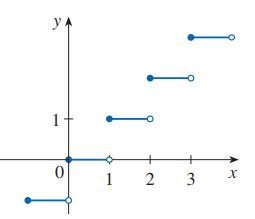
\includegraphics[width=3.5cm]{Jump.png}\\
            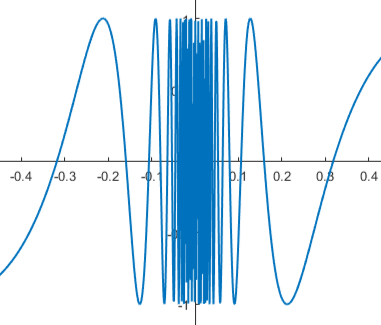
\includegraphics[width=4cm]{Oscillate.png}\\
        \end{multicols}
    \end{enumerate}

%%%%%%%%%%%%%%%%%%%%%%%%
%-------NEXTPAGE-------%
%%%%%%%%%%%%%%%%%%%%%%%%
    \newpage
    
    %IVT%
    \item Intermediate Value Theorem (I.V.T.)\\
    $$Assume\ f(x)\ is\ continuous\ on\ [a,b],$$
    $$\exists\ c\ \in[a,b],\  s.t.\ f(c)=k,\ f(a)<k<(b)$$

    %Limit at Infinity%
    \item Limits at Infinity\\
    General form: 
    \begin{equation}
        \lim\limits_{x\to\infty}\frac{a_{m}x^{m}+a_{m-1}x^{m-1}+...+a_{0}x^{0}}{b_{n}x^{n}+b_{n-1}x^{n-1}+...+b_{0}x^{0}}=
        \left\{
        \begin{aligned}
        \infty(-\infty),\ &m>n \\
        \frac{a_m}{b_n},\ &m=n \\
        0,\ &m<n
        \end{aligned}
        \right.\nonumber
    \end{equation}

    Expansion speed: $n^n > n! > a^n > n^a > ln(n)$\\
    
    %Asymptotes%
    \item Asymptotes
    \begin{enumerate}[(1)]
        
        %HA%
        \item Horizontal Asymptotes (H.A.)\\
        H.A. $\Rightarrow$ Occurs when $x$ approaches $\pm\infty$.\\ 
        So let $x$ approaches $\pm\infty$ can find whether the function has horizontal asymptotes.\\
        Ex. Find the asymptotes of $f(x)=e^{-x}$\\
        \begin{equation}
            \begin{aligned}
                \lim\limits_{x\to\infty}e^{x}&=\infty\\
                \lim\limits_{x\to-\infty}e^{x}&=0\hspace{36em}
            \end{aligned}\nonumber
        \end{equation}
        
        %VA%
        \item Vertical Asymptotes (V.A.)\\
        V.A. $\Rightarrow$ Occurs at $f(x)$ approaches $\pm\infty$.\\
        So find the points where $f(x)$ approaches $\pm\infty$, that is the position of vertical asymptotes.\\
        Ex. Find the asymtote of $f(x)=\frac{1}{x}$\\
        \hspace*{2em}$f(x)$ approaches $\infty$ as $x$ approaches $0^+$, and approaches $-\infty$ as $x$ approaches $0^-$
        \\
        
        %SA%
        \item Slant asymptotes (S.A.)\\
        Methods to check the slant asymptotes of a function is as following:\\
        Method 1: Rationalization\\
        Ex. Find the asymtote of $f(x)=\frac{3x^2+2x+1}{x+3}$\\
        \begin{equation}
            \begin{aligned}
                f(x)&=\frac{3x^2+2x+1}{x+3}=(3x-7)+\frac{22}{x+3}\\
                \lim\limits_{x\to\infty}f(x)&=\lim\limits_{x\to\infty}[(3x+7)+\frac{22}{x+3}]\hspace{26em}\\
            \end{aligned}\nonumber\\
        \end{equation}
        \\
        Method 2: Derivative\\
    \end{enumerate}

    %Example and Exercise%
    \item Examples and Exercises
    \begin{enumerate}[(1)]

        %Continuity%
        \item Continuity\\
        Example:\\
        Show that the following function is continuous on $(-\infty, \infty)$.
        \begin{equation}
            f(x)=\left\{
            \begin{aligned}
                    &x^3sin(\frac{1}{x}), &if&\ x\neq 0\\
                    &0, &if&\ x=0\hspace{32em}         
                \end{aligned}    
            \right.\nonumber
        \end{equation}\\
        Exercise:\\
        Where is the following function continuous?
        \begin{equation}
            f(x)=\left\{
            \begin{aligned}
                    &tan(\frac{\pi}{4})x, &if&\ \left | x\right |<1\\
                    &x, &if&\ \left | x\right |\geqslant 1\hspace{32em}         
                \end{aligned}    
            \right.\nonumber
        \end{equation}\\

        %IVT%
        \item Intermediate Value Theorem\\
        Prove that the equation $\frac{x-1}{x^2+2}=\frac{3-x}{x+1}$ is solvable.
        \\
        \\
        \\
        \\
        \\
        \\
        %Infinite Limit%
        \item Infinite Limit
        \begin{multicols}{2}
            \begin{enumerate}
                \item $\lim\limits_{x\to\infty}cos^{-1}(\sqrt{x^2+x}-x)$\\
                \item $\lim\limits_{x\to\infty}\frac{4x^5+3x^2+2}{7x^5+3}$\\
                \item $\lim\limits_{x\to\infty}\frac{2\cdot5^x-3\cdot2^x}{7\cdot5^x+2\cdot4^x}$\\
                \item $\lim\limits_{x\to\infty}\frac{5^x}{x!}$\\
                \item $\lim\limits_{x\to\infty}x^{\frac{1}{x!}}$\\
            \end{enumerate}
            \begin{enumerate}
                \item $\lim\limits_{x\to\infty}(\sqrt{x^2+ax}-\sqrt{x^2+bx})$\\
                \item $\lim\limits_{x\to\infty}\frac{2(1/5)^x-3(1/3)^x}{7(2/3)^x+2(1/5)^x}$\\
                \item $\lim\limits_{x\to\infty}\frac{\sqrt{9x^2+1}}{x+4}$\\
                \item $\lim\limits_{x\to\infty}\frac{x^{2000}(\ln{x})^2}{e^x}$\\
                \item $\lim\limits_{x\to\infty}\sqrt[x]{x}$\\
            \end{enumerate}
        \end{multicols}

%%%%%%%%%%%%%%%%%%%%%%%%
%-------NEXTPAGE-------%
%%%%%%%%%%%%%%%%%%%%%%%%
        \newpage
        
        %Asymptotes%
        \item Asymptotes\\
        Find the horizontal and vertical asymptotes for the function, $f(x)=tan^{-1}({\frac{x-1}{x+1}})$\\
        \\
        \\
        \\
        \\
        \\
        Find all asymptotes of the following function $f(x)=\frac{x^3+4}{x^2}$\\
        \\
        \\
        \\
        \\
        \\
        
        %Curve Sketching%
        \item Curve sketching\\
        \hspace*{2em} Plot the graph satisfying the following conditions,\\
        \begin{equation}
            \left\{
            \begin{aligned}
                &\lim\limits_{x\to\pm\infty}=0\\
                &\lim\limits_{x\to3^-}\ \,=-\infty\\
                &\lim\limits_{x\to3^+}\ \,=\infty
            \end{aligned}
            \right.\nonumber\hspace{36em}
        \end{equation}
    \end{enumerate}

\end{enumerate}
\end{document}